When it comes to blackbox attacks, two existing approaches are evaluated: the Transfer based approach and the Boundary attack.

In the transfer based approach, I take 1000 samples that are previously unseen to target neural network and obtain labels for them by querying the target neural network. Then a substitute network that is pretrained on the ImageNet dataset is trained on those 1000 samples with labels that are obtained from the target network. The idea of such a process is to achieve the similar decision boundaries for the substitute network as they are in the targeted network.

Next, I take random 100 samples that are yet unseen by both networks and evaluate  MAE of the targeted neural network and the substitute network on those 100 images. Then I craft adversarial samples for the substitute neural network using those 100 images. Target labels for adversarial samples are set in the same manner as in whitebox attacks. Finally, I evaluate MAE of the targeted neural network and the substitute network on those 100 adversarial samples.

Results are presented in Tables \ref{table:bbox-fgsm-resnet} and \ref{table:bbox-cw-resnet}.


\begin{table}[]
\begin{tabular}{|c|c|c|c|c|}
\hline
 & \multicolumn{2}{c|}{Clean Samples} & \multicolumn{2}{c|}{Adversarial samples} \\ \hline
Target model id & Blackbox MAE & Substitute MAE & Blackbox MAE & Substitute MAE \\ \hline
1 & 6.21 & 14.17 & 6.61 & 14.20 \\ \hline
2 & 8.61 & 13.20  &  8.17 & 13.39  \\ \hline
3 & TODO & TODO  & TODO & TODO  \\ \hline
4 & TODO & TODO & TODO & TODO \\ \hline
\end{tabular}
\caption{Results using the ResNet-50 architecture for the substitute network and FGSM attack for crafting adversarial samples for it}
\label{table:bbox-fgsm-resnet}
\end{table}


\begin{table}[]
\begin{tabular}{|c|c|c|c|c|}
\hline
 & \multicolumn{2}{c|}{Clean Samples} & \multicolumn{2}{c|}{Adversarial samples} \\ \hline
Target model id & Blackbox MAE & Substitute MAE & Blackbox MAE & Substitute MAE \\ \hline
1 & 6.21 & 15.92 & 6.10 & 15.93 \\ \hline
2 &  TODO & TODO  & TODO &  \\ \hline
3 &  TODO & TODO  & TODO &  \\ \hline
4 &  TODO & TODO  & TODO &  \\ \hline
\end{tabular}
\caption{Results using the ResNet-50 architecture for the substitute network and CW attack for crafting adversarial samples for it}
\label{table:bbox-cw-resnet}
\end{table}

When it comes to the boundary attack, it's hard to do any quantitative analysis because the attack, as described in Section \ref{sec:boundary-attack}, is fundamentally different that the transfer based approach. Instead, I generate several samples and discuss them. One sample can be seen in Figure \ref{fig:trump-adv} and the corresponding results in \ref{fig:trump-softmax}. TODO: ADD reference to other images. The other samples can be found in Appendix. discussion follows in the chapter TODO.


\begin{figure}
\begin{subfigure}{.5\textwidth}
  \centering%
  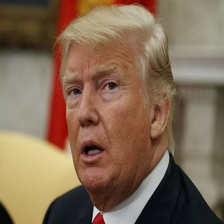
\includegraphics[height=5cm, width=\linewidth, keepaspectratio]{image0.jpg}
  \caption{The starting image}
\end{subfigure}
\begin{subfigure}{.5\textwidth}
  \centering
  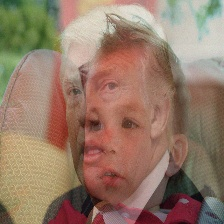
\includegraphics[height=5cm, width=\linewidth, keepaspectratio]{image1000.jpg}
  \caption{1000 queries}
\end{subfigure}

\begin{subfigure}{.5\textwidth}
  \centering
  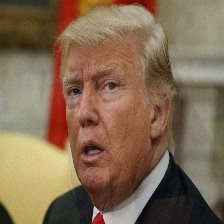
\includegraphics[height=5cm, width=\linewidth, keepaspectratio]{image2000.jpg}
  \caption{2000 queries}
\end{subfigure}
\begin{subfigure}{.5\textwidth}
  \centering
  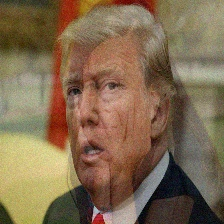
\includegraphics[height=5cm, width=\linewidth, keepaspectratio]{image4000.jpg}
  \caption{4000 queries}
\end{subfigure}

\begin{subfigure}{.5\textwidth}
  \centering
  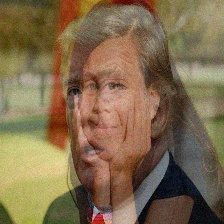
\includegraphics[height=5cm, width=\linewidth, keepaspectratio]{image8000.jpg}
  \caption{8000 queries}
\end{subfigure}
\begin{subfigure}{.5\textwidth}
  \centering
  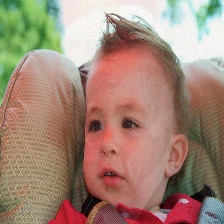
\includegraphics[height=5cm, width=\linewidth, keepaspectratio]{image12000.jpg}
  \caption{12000 queries}
\end{subfigure}

\begin{subfigure}{.5\textwidth}
  \centering
  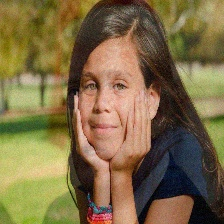
\includegraphics[height=5cm, width=\linewidth, keepaspectratio]{image16000.jpg}
  \caption{16000 queries}
\end{subfigure}
\begin{subfigure}{.5\textwidth}
  \centering
  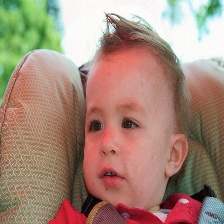
\includegraphics[height=5cm, width=\linewidth, keepaspectratio]{final_adversarial.jpg}
  \caption{Final adversarial sample}
\end{subfigure}
\caption{Although an adversary is changing the image, the blackbox classifier is not changing the prediction (68 years old)}
\label{fig:trump-adv}
\end{figure}

\begin{figure}
\begin{subfigure}{.5\textwidth}
  \centering
  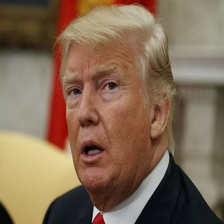
\includegraphics[height=5cm, width=\linewidth, keepaspectratio]{image0.jpg}
  \caption{Starting image}
\end{subfigure}
\begin{subfigure}{.5\textwidth}
  \centering
  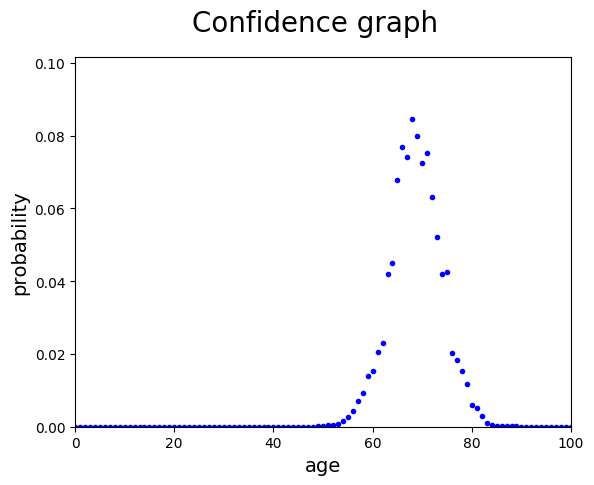
\includegraphics[height=5cm, width=\linewidth, keepaspectratio]{softmaxbenign.png}
  \caption{Predictions for the starting image}
\end{subfigure}
\caption{Starting image and the corresponding prediction}
\label{fig:starting-image-softmax}
\end{figure}

\begin{figure}
\begin{subfigure}{.5\textwidth}
  \centering
  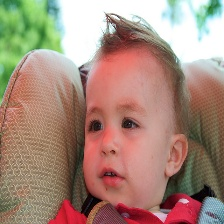
\includegraphics[height=5cm, width=\linewidth, keepaspectratio]{source_image.jpg}
  \caption{The targeted image}
\end{subfigure}
\begin{subfigure}{.5\textwidth}
  \centering
  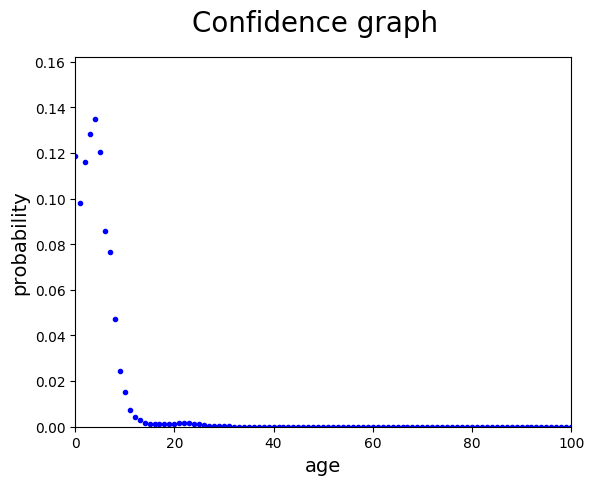
\includegraphics[height=5cm, width=\linewidth, keepaspectratio]{softmaxsource_image.png}
  \caption{Predictions for the targeted image}
\end{subfigure}

\caption{Targeted image and the corresponding predictions}
\label{fig:targeted-image-softmax}
\end{figure}

\begin{figure}

\begin{subfigure}{.5\textwidth}
  \centering%
  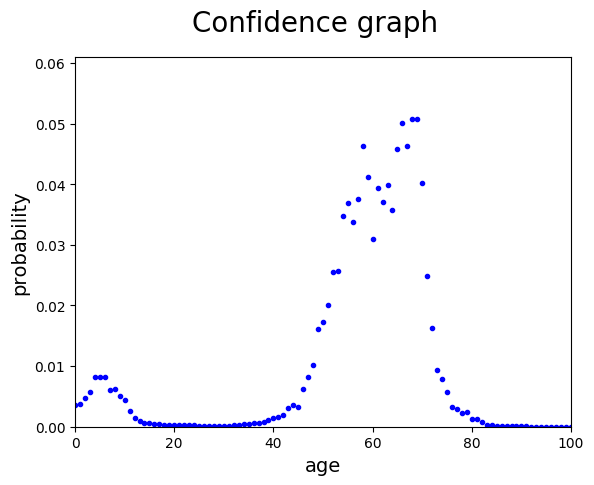
\includegraphics[height=5cm, width=\linewidth, keepaspectratio]{softmax3000.png}
  \caption{3000 queries}
\end{subfigure}
\begin{subfigure}{.5\textwidth}
  \centering%
  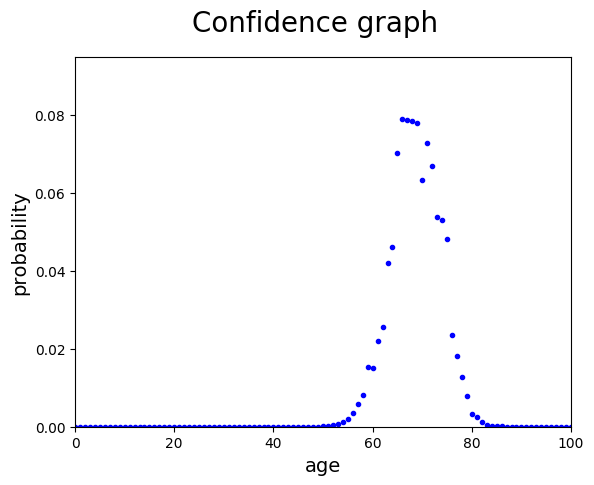
\includegraphics[height=5cm, width=\linewidth, keepaspectratio]{softmax4000.png}
  \caption{4000 queries}
\end{subfigure}


\begin{subfigure}{.5\textwidth}
  \centering%
  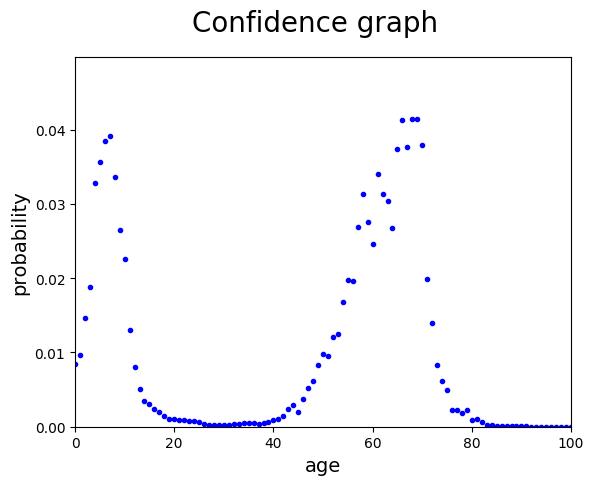
\includegraphics[height=5cm, width=\linewidth, keepaspectratio]{softmax8000.png}
  \caption{8000 queries}
\end{subfigure}
\begin{subfigure}{.5\textwidth}
  \centering%
  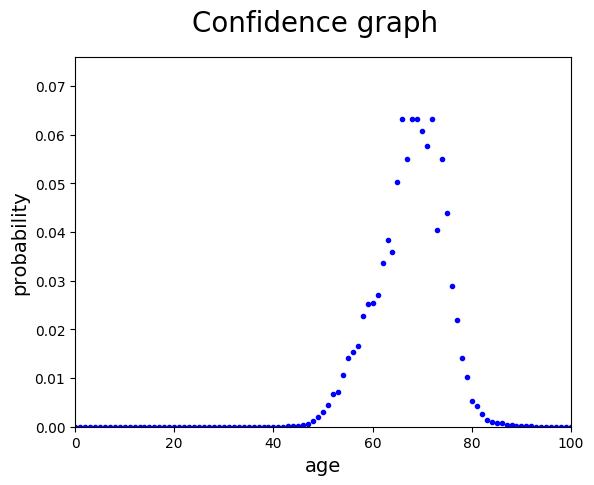
\includegraphics[height=5cm, width=\linewidth, keepaspectratio]{softmaxadversarial.png}
  \caption{The final adversarial sample (77 000 queries)}
\end{subfigure}

\caption{Predictions of the blackbox classifier for images corresponding to Figure \ref{fig:trump-adv}. In all the graphs, age 68 is predicted with the maximum probability.}
\label{fig:trump-softmax}
\end{figure}


